\scanpage{45}
% Printed sheet upside down in the scan; transcribed after 180-degree rotation.
% One long diagonal cancellation stroke crosses the reused letter.
\deleted{
UNIVERSITE\\
DES SCIENCES ET TECHNIQUES\\
\uline{DU LANGUEDOC}\\
JFR/MD

Montpellier, le 22 Juin 1978

LE DIRECTEUR DE L'U. E. R. III

à

Mesdames et Messieurs les Membres\\
des Jurys des examens de l'U.E.R. III

Madame, Monsieur,

Le Conseil de l'U.E.R. III se permet de vous rappeler\\
qu'une réforme des maîtrises spécialisées est en cours, et que\\
tous les dossiers d'habilitation ou de reconduction devront parve-\\
nir au Ministère avant le 31 janvier 1979.

Pour faciliter sa tâche il vous serait reconnaissant de\\
bien vouloir lui indiquer si vous désirez que la maîtrise où vous\\
enseignez soit reconduite ou si vous souhaitez la modifier en tout\\
ou partie.

Il a pensé que les Jurys des différents certificats\\
étaient les plus propres à diffuser cette lettre auprès des ensei-\\
gnants qui s'estiment concernés. Il espère qu'ils voudront bien\\
examiner attentivement ce problème.

Il accueillera toute suggestion dont vous pourriez lui\\
faire part avant le 15 octobre 1978.

Il compte sur votre aide et vous prie de croire à tout\\
son dévouement.

Le Directeur de l'U.E.R. III,
\figure{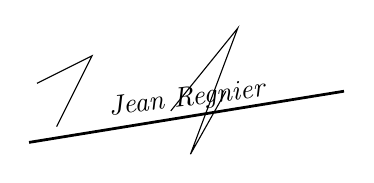
\begin{tikzpicture}[x=1cm,y=1cm]
\node[font=\itshape,rotate=7] at (2,.4) {\unsure{Jean Regnier}};
\draw[line width=1pt] (0,-.15)--(4,.5);
\draw (.1,.6)--(.8,.95)--(.35,.05);
\draw (1.8,.25)--(2.65,1.3)--(2.05,-.3)--(2.5,.5);
\end{tikzpicture}}
\uline{J.F. REGNIER}

\uline{N.B.} : Cette lettre a été transmise pour information aux Directeurs\\
d'U.E.R. et aux Membres du Conseil de l'U.E.R. III.
}
% archive foliation: 44
